\documentclass[tikz,border=0cm]{standalone}

\usepackage{amsmath,amssymb,amsfonts}
\usetikzlibrary{calc,
fit,
shapes.misc,
shapes.geometric,
arrows.meta,
fadings,
matrix,
chains,
scopes,
positioning}

\usepackage{pgfplots}
\usepackage{pgfplotstable}
\pgfplotsset{compat=1.18}



\usepackage[]{fontspec}

\setmainfont{Latin Modern Roman}
\setmonofont{Latin Modern Math}
\renewcommand{\textsc}[1]{{\fontfamily{lmr}\selectfont \scshape #1}}

\usepackage[]{bm}

\makeatletter
\@ifundefined{fromRoot}{\newcommand{\fromRoot}[1]{../../#1}}{}

\def\input@path{{../..}{..}{.}{./svg}{./pgfplots}{./tikzpicture}}
%or: \def\input@path{{/path/to/folder/}{/path/to/other/folder/}}
\makeatother

\newcommand*{\gf}[1]{\acrshort{gf}($#1$)}%
\newcommand*{\mpn}[1]{\bm{P}_{#1}}%
\newcommand*{\pn}[1]{%
  \ifthenelse{\equal{#1}{}}{$\mpn{0}$}{$\mpn{#1}$}%
}%

\newcommand*{\pk}[3]{%
  \ifthenelse{\equal{#1}{#2}}{\textcolor{red}{\phantom{.}$p_0$\phantom{.}}}{\phantom{.}$p_#3$\phantom{.}}%
}%


\newcommand*{\placeholder}{
\includegraphics[width=\linewidth, height=.25\textheight, keepaspectratio = true]{figures/certified_xilinx.png}}%

\newcommand*{\snr}{\acrshort{snr}}%
\newcommand*{\snrs}{\acrshortpl{snr}}%

\newcommand*{\mpd}[0]{p_\Delta}%
\newcommand*{\mpo}[0]{p_\omega}%
\newcommand*{\pd}[0]{$\mpd$}%
\newcommand*{\po}[0]{$\mpo$}%
\newcommand*{\mpfa}[0]{\mathcal{P}_{fa}}%
\newcommand*{\mpmd}[0]{\mathcal{P}_{md}}%
\newcommand*{\pfa}[0]{\acrshort{pfa}}%
\newcommand*{\pmd}[0]{\acrshort{pmd}}%
\newcommand*{\mnorm}[1]{\mathcal{L}_{#1}}%
\newcommand*{\norm}[1]{$\mnorm{#1}$}%
\newcommand*{\fft}{\acrshort{fft}}%
\newcommand*{\mfft}[1]{\mathcal{F}(#1)}%
\newcommand*{\mifft}[1]{\mathcal{F}^{-1}(#1)}%
\newcommand*{\ts}{\acrshort{ts}}%

\newcommand*{\cpp}[1]{C\textrm{++#1}}%
\newcommand*{\na}{\textrm{\textcolor{SlateGray4}{N/A}}}%

\newcommand*{\vect}[1]{\bm{#1}}%
\newcommand*{\mat}[1]{\bm{\mathrm{#1}}}%

\newcommand*{\task}[1]{\mathcal{T}_{#1}}%

\newcommand*{\sdr}{\acrshort{sdr}}%
\newcommand*{\fpga}{\acrshort{fpga}}%



\usetikzlibrary{calc, shapes.misc, shapes.geometric, arrows.meta, positioning, overlay-beamer-styles, fit}

\begin{document}

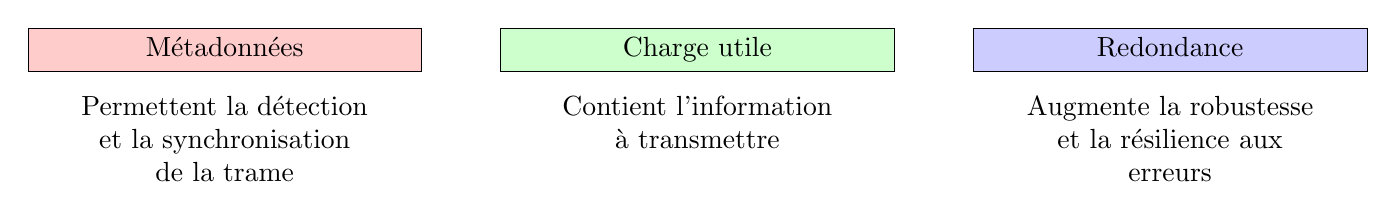
\begin{tikzpicture} [-latex,
        >=latex,
        auto,
        ultra thin,
        main node/.style={rectangle, fill = white!35,  draw,
                align=center}]
    

    \node [
        draw,
        fill = red!20!white,
        minimum width = 5 cm,
    ] (meta) at (0, 0) {\phantom{g}Métadonnées\phantom{g}};

    \node [
        draw,
        fill = green!20!white,
        minimum width = 5 cm,
        right = 1 cm of meta
    ] (data)  {Charge utile};

    \node [draw,
        fill = blue!20!white,
        minimum width = 5 cm,
        right = 1 cm of data
    ] (ecc)  {\phantom{g}Redondance\phantom{g}};

    \node [
        align = center,
        below = 2 mm of meta
    ] (meta_leg)  {Permettent la détection\\et la synchronisation\\de la trame};

    \node [
        align = center,
        below = 2 mm of data
    ] (data_leg)  {Contient l'information\\à transmettre};

    \node [
        % minimum width = 8 cm,
        align = center,
        below = 2 mm of ecc
    ] (ecc_leg)  {Augmente la robustesse\\et la résilience aux\\erreurs};

\end{tikzpicture}
\end{document}
